\documentclass[journal,letterpaper]{IEEEtran}
\usepackage[T1]{fontenc}
\usepackage[utf8]{inputenc}
\usepackage{newtxtext,newtxmath}
\usepackage{cite,booktabs,array,tabularx,tikz,placeins,xurl,graphicx}
\usetikzlibrary{arrows.meta,positioning}
\usepackage[hidelinks,breaklinks]{hyperref}
\hypersetup{pdftitle={GridMind: Graduation Project Proposal, Sections I and II},pdfsubject={Introduction and Review Protocol and Methodology}}
\setlength{\emergencystretch}{1.5em}
\raggedbottom
\makeatletter
\def\ps@gridmind{%
  \def\@oddhead{\fontsize{7}{8}\selectfont MISR INTERNATIONAL UNIVERSITY/FACULTY OF COMPUTER SCIENCE, NOVEMBER 2026\hfil\thepage}%
  \let\@evenhead\@oddhead\def\@oddfoot{}\let\@evenfoot\@oddfoot}
\let\ps@plain\ps@gridmind
\let\ps@headings\ps@gridmind
\let\ps@IEEEtitlepagestyle\ps@gridmind
\newenvironment{inlinetable}{\par\medskip\noindent\begin{minipage}{\columnwidth}\def\@captype{table}}{\end{minipage}\par\medskip}
\setlength{\@fptop}{0pt}
\setlength{\@dblfptop}{0pt}
\makeatother
\hyphenation{Grid-Mind synchro-phasor repro-ducibility}
\markboth{MISR INTERNATIONAL UNIVERSITY/FACULTY OF COMPUTER SCIENCE, NOVEMBER 2026}{MISR INTERNATIONAL UNIVERSITY/FACULTY OF COMPUTER SCIENCE, NOVEMBER 2026}
\title{A Graduation Project Proposal on\\GridMind: AI Decision Support for Power Grids}
\author{}
\begin{document}
\maketitle
\pagestyle{gridmind}\thispagestyle{gridmind}

\section{Introduction}
Reliable electricity supports households, public services, and economic activity. In Egypt, renewable-energy integration is accompanied by investment in the transmission infrastructure that carries power between generation sites and demand centers. The European Investment Bank's Egypt Grid Modernization and Expansion project supports grid development to accommodate renewable generation~\cite{EIB}. The European Bank for Reconstruction and Development's NWFE Electricity Grid Reinforcement project includes a Cairo substation upgrade and a transmission line connecting renewable generation from the Gulf of Suez region~\cite{EBRD}. These initiatives provide a national motivation for investigating software that helps engineers interpret operating information and assess possible responses alongside physical network development.

Power-system decision support involves several related questions. Engineers need usable measurements of the current state, estimates of future demand and renewable production, an interpretation of abnormal signals, and an assessment of how an outage could affect other components. A useful response must also respect the network's electrical and operating limits. Missing values, forecast errors, and ambiguous measurements influence these decisions in different ways. A missing reading can arise while equipment remains in service, whereas a physical outage changes the network itself. Similarly, a forecast of aggregate demand or solar generation does not directly identify which transmission line will become overloaded. These distinctions shape the information that an integrated platform must exchange.

Research offers several approaches to recovering incomplete operating information. P. Li et al. use a spatio-temporal dynamic graph neural network to recover missing measurements for state estimation~\cite{S28}. B. Li et al. reconstruct PMU voltage phasors using a K-hop graph network and auxiliary low-rank learning under incomplete observability~\cite{N01}. Wei et al. combine physics-guided graph learning with online data fusion for distribution-system measurement recovery~\cite{S29}. Their inputs and assumptions differ: line-terminal power measurements, bus-voltage phasors, and distribution measurements cannot be treated as interchangeable targets. These studies motivate preserving measurement identity, topology, and the distinction between observed and reconstructed values.

Forecasting studies address the changing balance between demand and renewable generation. Bolusteve et al. compare direct net-load prediction with an indirect method that forecasts demand, wind, and solar output separately, using one-hour-ahead ERCOT data~\cite{S25}. Voyant et al. investigate efficient multi-output short-term forecasting~\cite{S20}, while H. Wang et al. use variable attention and multi-task learning to exploit relationships among wind, solar, and load series~\cite{S24}. The methods provide alternatives for representing related targets, but differences in horizon, geographic setting, and available inputs affect their relevance to a common experiment. For GridMind, separate forecasts would retain the three physical quantities and allow net load to be derived explicitly.

Abnormal-event diagnosis requires separating problems in the measurements from changes in the electrical system. Khare et al. detect and correct false PMU data using relationships learned across measurements~\cite{S10}. Veerakumar et al. examine bad-data discrimination and sudden load changes within forecasting-aided state estimation~\cite{S18}. For physical disturbances, Shadi et al. connect detection, classification, and localization in a hierarchical framework~\cite{S11}, and Riaz et al. investigate staged machine-learning and deep-learning diagnosis~\cite{S16}. These contributions support a staged design, while also showing why measurement-error labels, fault categories, and location targets must be specified separately. Evaluation should distinguish event episodes from correlated samples and classification performance from localization error~\cite{S12}.

Cascade assessment and corrective operation concern the consequences of an abnormal state and the available interventions. Qin et al. combine graph attention, temporal learning, and self-supervision for cascading-fault prediction in AC/DC test settings~\cite{N02}. Ghasemi et al. learn conditional interactions among line failures~\cite{S02}, whereas Rivas-Davalos et al. rank critical lines using weighted natural connectivity~\cite{S03}. A criticality ranking, a conditional line-failure prediction, and a time-dependent failure trajectory represent different outputs. For corrective operation, Moaidi and Bessa learn operating rules in a Grid2Op congestion-management environment~\cite{S08}; Gautam et al. optimize generator redispatch~\cite{S09}. Action spaces and physical checks determine whether either approach can inform the proposed response mechanism.

Existing integration research further connects predictions with operating decisions. G. Wang et al. argue for decision-aware learning that accounts for the effect of prediction errors on optimization~\cite{S37}. Worou et al. link cascade-aware risk assessment, intervention cost, and operational-impact proxies in a benchmark maintenance framework~\cite{S38}. The learning-based optimal-power-flow review by Khaloie et al. also distinguishes solution quality, constraint feasibility, and computational performance~\cite{S05}. These sources support evaluating the consequences of a recommendation alongside the accuracy of its underlying models. Their results do not establish performance for a platform combining GridMind's specific tasks and controls.

The research gap addressed by this study is the evidence needed to connect these capabilities under consistent information and evaluation assumptions. Specialized models and partially integrated frameworks already exist. Their datasets, measurement channels, horizons, topologies, and available controls nevertheless differ. Combining them requires explicit decisions about timestamps, units, component identifiers, uncertainty, and how errors affect later stages. A structured literature review is therefore needed to compare suitable approaches, identify reusable evidence, and establish requirements for the proposed system without equating performance across incompatible experimental settings.

GridMind is proposed as a software-based, human-in-the-loop platform combining missing-telemetry reconstruction, demand and renewable forecasting, event diagnosis, cascade-risk prediction, and corrective-action recommendation. The platform would retain quality flags on reconstructed readings, produce one-hour-ahead demand, solar, and wind forecasts, distinguish measurement problems from physical abnormalities, and assess cascade consequences for defined initiating outages. Candidate corrective actions would be compared through power-flow and operating-constraint checks before presentation to an engineer. A shared network representation and dashboard would connect these outputs while preserving their assumptions and provenance.

The initial evaluation will use public time series and benchmark or simulated power networks. Forecasts will be mapped into network operating scenarios through declared allocation and scaling assumptions. Egypt provides the application motivation; operational transfer would require representative local data and assessment with electricity-sector specialists. The project objectives are to synthesize the evidence across the five capabilities, select methods and task-appropriate baselines, define compatible interfaces, and evaluate both individual outputs and their usefulness within the integrated workflow. Intended improvements in accuracy, response time, and decision quality remain evaluation goals.

The review is guided by the following research questions:
\begin{itemize}
\item \textbf{RQ1 (State of the Art):} What research and solutions exist for AI-based telemetry reconstruction, demand and renewable forecasting, event diagnosis, cascade-risk prediction, and corrective-action recommendation?
\item \textbf{RQ2 (Methods):} Which models, datasets, technologies, and evaluation approaches support these capabilities, and what tradeoffs do they present?
\item \textbf{RQ3 (Market \& Tools):} Which academic prototypes, commercial platforms, and open-source tools support these tasks, and how do their capabilities, accessibility, and costs compare?
\item \textbf{RQ4 (Gaps):} What challenges remain in data quality, generalization, reproducibility, integration, and physical validation?
\item \textbf{RQ5 (Proposed Directions):} What evidence-based improvements could address these gaps through an integrated platform relevant to Egypt's electricity-modernization context?
\end{itemize}
Section II describes the review methodology. Section III synthesizes answers to RQ1--RQ5. Section IV interprets the findings and develops the conceptual framework, and Section V examines threats to validity. Section VI presents the proposed solution and its design rationale. Section VII concludes with the principal findings and their research and practical implications.

\section{Review Protocol and Methodology}
This structured literature review examines the evidence supporting GridMind's five capabilities and their integration. Its organization draws on Kitchenham and Charters' review guidance~\cite{Kitchenham}, with study-selection reporting informed by PRISMA 2020~\cite{PRISMA}. Searches were divided among members according to their assigned models. Candidate papers were reviewed and approved by the supervisor. A focused synthesis then selected complementary evidence for the project's technical decisions and evaluation requirements.

\subsection{Eligibility Criteria}
The inclusion criteria were:
\begin{itemize}
\item English-language studies relevant to at least one GridMind capability or to integrated power-system decision support.
\item Research published during 2021--2026, including journal articles and relevant preprints, with publication type identified when interpreting the evidence.
\item Empirical studies describing their methods, datasets or simulation cases, and evaluation, together with reviews that provide a relevant methodological synthesis.
\item Studies contributing a direct task match, a useful baseline, an evaluation framework, or complementary evidence for integration.
\end{itemize}
The exclusion criteria were unrelated application targets, duplicate study records, inaccessible full texts, and descriptions insufficient to assess the claimed method or evidence. Additional relevant studies could remain background references when their contribution overlapped with the focused comparison or addressed a narrower application.

Dataset identity and accessibility were examined during selection. Public data, simulated benchmark cases, and restricted research datasets were distinguished. Restricted or unavailable datasets were recorded as reproducibility limitations rather than automatic exclusion criteria. For reviews, the evidence consists of the reviewed literature rather than a newly generated training dataset. A paper's accessible full text and the availability of its underlying dataset were assessed separately.

\subsection{Search Strategy}
Searches used ScienceDirect and Springer Nature Link to identify research on the five capabilities and integrated decision support. Terms combined power-system terminology with the target task. Publication-year, article-type, subject, discipline, and open-access filters were used according to the search. The reported search expressions were:
\begin{enumerate}
\item \texttt{Cascading failure prediction in power systems using machine learning}
\item \texttt{("power system" OR "power grid") AND ("missing measurements" OR "measurement reconstruction" OR "data imputation")}
\item \texttt{Power system event classification and fault localization using machine learning}
\item \texttt{"cascading failures" AND "transmission lines"}
\item \texttt{(wind AND (solar OR photovoltaic) AND (load OR demand)) AND ("net load" OR "short-term forecasting")}
\item \texttt{"smart grid" AND "decision support system" AND "artificial intelligence"}
\item \texttt{Power System OR Power Grid AND Corrective Action OR Corrective Control AND Artificial Intelligence}
\item \texttt{"power grid" AND "digital twin" AND "decision making"}
\item \texttt{"synchrophasor" AND ("bad data" OR "measurement anomalies" OR "clock errors") AND ("grid events" OR "disturbance")}
\end{enumerate}
The expressions cover measurement recovery, physical events and measurement anomalies, forecasting, cascade propagation, corrective control, and integration. Across the nine reported queries, the initial results totalled 18,519 search occurrences. Recorded totals decreased to 15,607 after date filtering, 9,563 after article-type filtering, 3,624 after subject/discipline and open-access filtering, and 2,133 in the final-search column. These totals describe query results and can include the same paper in more than one search. Search results were examined for datasets and benchmark networks, target compatibility, and evaluation evidence. Dataset names, source references and accessibility were recorded for each empirical study. Access restrictions were considered when assessing reproducibility and suitability for implementation.

\subsection{Study Selection Process}
Study selection involved three activities:
\begin{enumerate}
\item \textit{Module-based screening:} Each member searched for papers relevant to the assigned models and examined titles, abstracts, methods, and application targets.
\item \textit{Supervisor review:} Candidate papers were submitted for supervisor approval, considering their relevance to the project.
\item \textit{Focused synthesis:} The 53-entry candidate list was assessed for direct relevance, complementary methods, dataset or benchmark evidence, and usefulness to the research questions. Twelve candidates were set aside during title and abstract screening because their targets were more specialized or already covered. The remaining 41 reports were available for full-text assessment. Twenty-three were set aside from the focused comparison: 16 for overlapping task, baseline or evaluation coverage and seven for specialized or broader scope. Eighteen studies were retained for detailed extraction.
\end{enumerate}
The selected studies cover three reconstruction papers, three forecasting papers, four diagnosis papers, three cascade papers, three corrective-action papers, and two integration papers. The four diagnosis studies cover measurement-error discrimination, staged physical-event analysis, affected-bus identification, and classifier/localization comparisons. Measurement-integrity and evaluation-framework references provide supporting context without adding extraction rows. Figure~\ref{fig:selection} presents the recorded keyword-search filtering alongside screening of the 53 candidate records. Search totals are result occurrences, while the candidate branch follows individual records through to the 18 selected studies. The final review count is taken from the candidate branch; the two branches are not added together.

\begin{figure*}[!t]
\centering
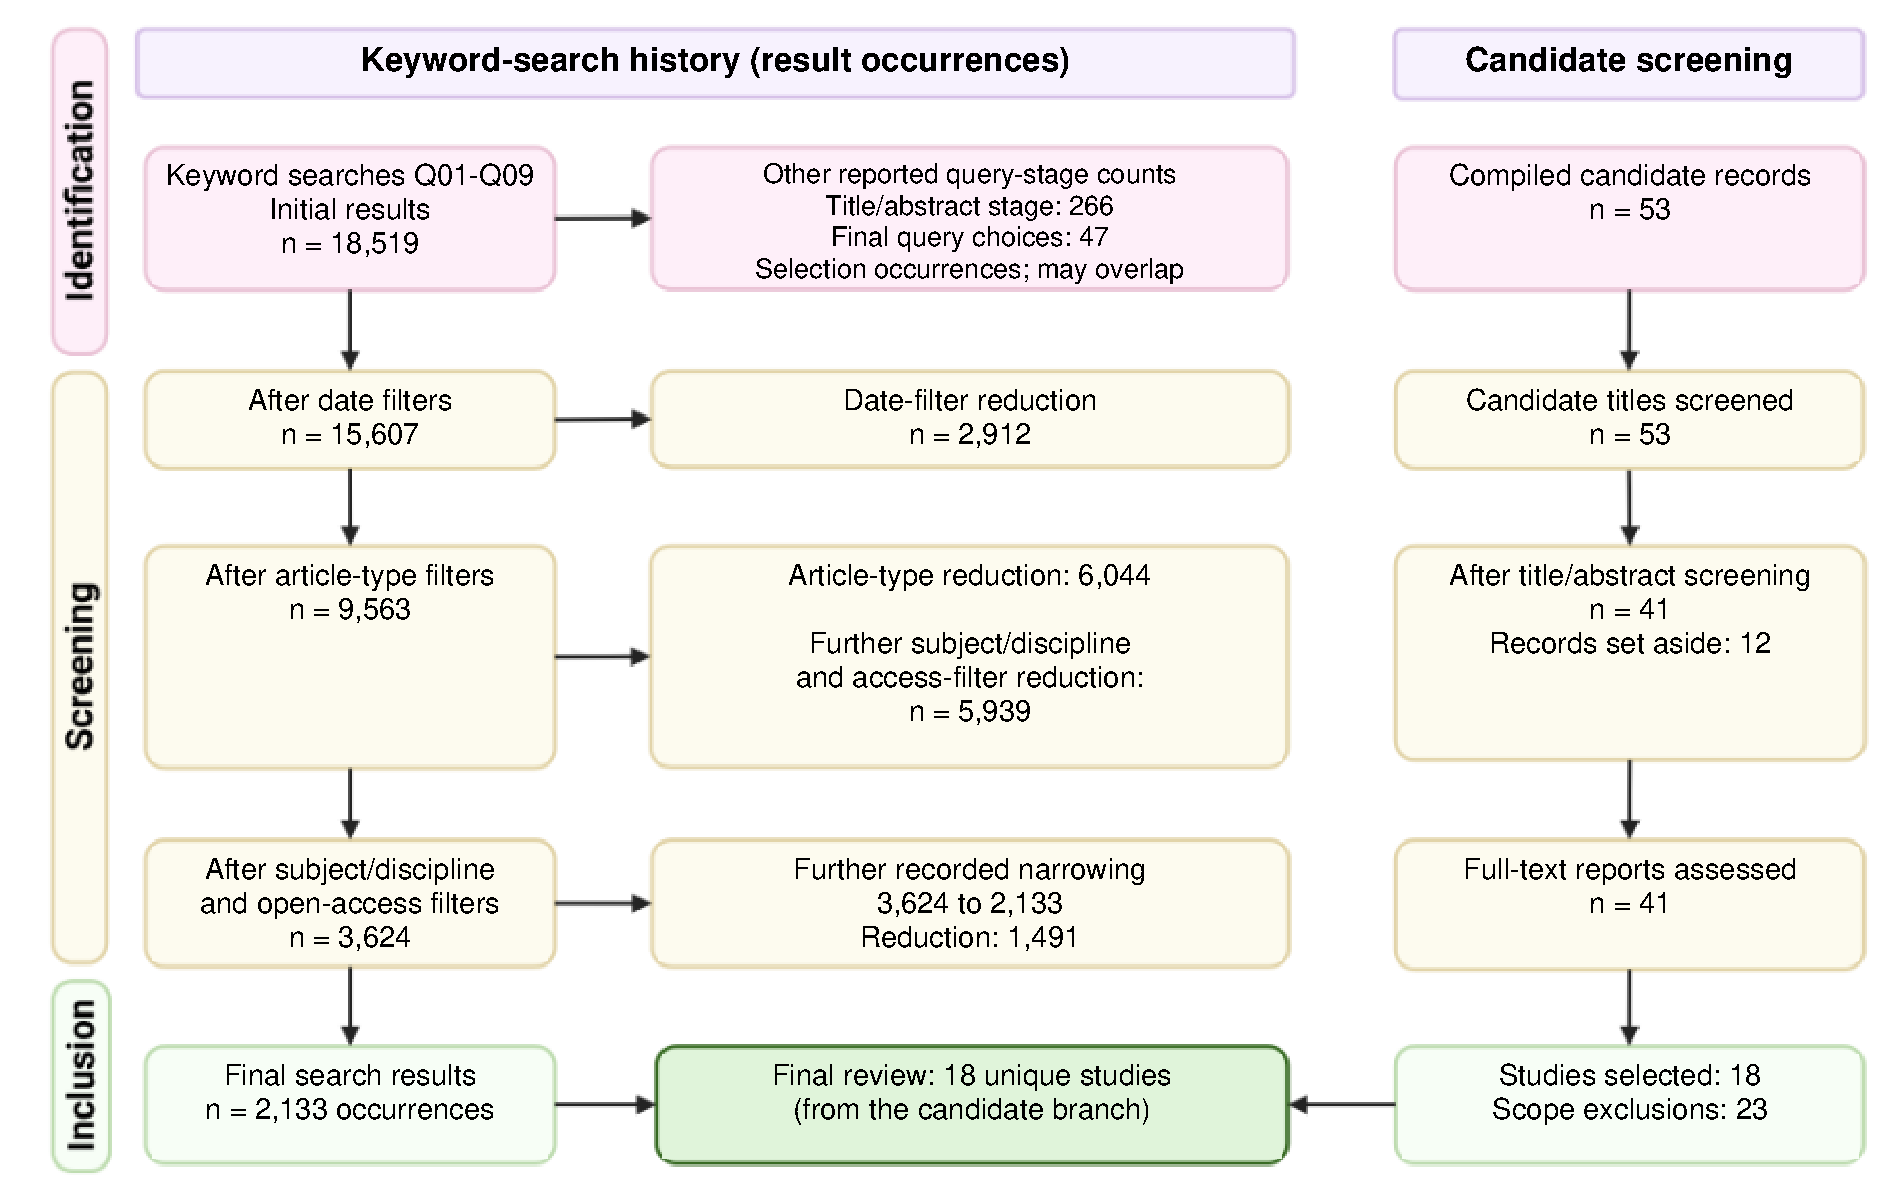
\includegraphics[width=\textwidth]{selection_figure.pdf}

\caption{PRISMA-style diagram of recorded keyword-search filtering and candidate selection. Search occurrences and candidate-study counts are reported separately.}
\label{fig:selection}
\end{figure*}

\subsection{Quality Assessment}
Each selected study was evaluated using a five-criterion checklist adapted from Kitchenham and Charters~\cite{Kitchenham}:
\begin{itemize}
\item Clarity of the research objectives.
\item Suitability of the proposed method for the task.
\item Transparency of the dataset and evaluation.
\item Reproducibility of the reported procedure.
\item Support for the findings and conclusions.
\end{itemize}
Each criterion was scored Yes = 1, Partial = 0.5, or No = 0. The study score is the mean of the five criteria. A mean below 0.5 is insufficient for inclusion in the focused synthesis. Dataset restrictions qualify reproducibility and are considered alongside the detail of the simulation or data-generation procedure.

The 18 selected studies scored between 0.70 and 1.00, with a mean of 0.87. All met the 0.50 threshold. Their final selection also considered direct relevance and complementary coverage. These scores assess the strength and reporting of the evidence, separately from predictive accuracy or other experimental performance metrics. Reviews were assessed for methodological synthesis and reporting rather than for producing a new training dataset.

\subsection{Data Extraction and Synthesis}
Extraction recorded authors, year, publication venue, domain, objective, model or technique, dataset or evidence, evaluation metrics, findings, and limitations. Dataset evidence identifies the named dataset or benchmark, relevant sample or scenario counts where reported, and its source. Access limitations are considered alongside the findings. Original dataset or repository references accompany named public resources in Table I. Each selected study has one extraction row. Input and output definitions were checked to distinguish direct implementation references from task-adjacent evidence. Preprints were identified separately from journal articles.

The extraction also considered task-specific requirements. Reconstruction records distinguish bus-voltage phasors, line-terminal power flows, missingness patterns, and the information available at reconstruction time. Forecasting records distinguish target quantities, horizons, chronological splits, and issue-time inputs. Diagnosis records distinguish sensor problems, physical fault types, location outputs, and episode-level evaluation. Cascade records distinguish critical-line ranking, conditional failure prediction, and temporal propagation. Corrective-action records distinguish switching, redispatch, curtailment, operating constraints, cost, and runtime.

Narrative and thematic synthesis first compares studies within each capability, then examines their interfaces and shared limitations. Findings retain their original dataset, network, horizon, and action-space context. Prediction errors from different experiments are not pooled into a common ranking. Integration evidence is examined for the connection between predictions and operational decisions, including the assumptions behind cost and unserved-energy measures. The synthesis supports the five research questions and the subsequent system design.

\subsection{Data Extraction Template (Longtable)}
Table I presents one row per selected paper using the template's bibliographic, methodological, evidence, and findings fields. Domain identifies the GridMind capability. LR Stage distinguishes quantitative empirical evidence from qualitative review synthesis. Dataset entries summarize the evidence used in each paper. The findings column records the principal contribution and limitations, including restricted access, simulated conditions, and differences from the proposed task. Numbered identifiers link each row to the reference list. Venue abbreviations include IJEPES for the International Journal of Electrical Power \& Energy Systems and EPSR for Electric Power Systems Research.
\begin{table*}[!t]
\caption{Data extraction form}
\centering\fontsize{8}{9.3}\selectfont\setlength{\tabcolsep}{2pt}
\begin{tabular}{>{\raggedright\arraybackslash}p{18pt}>{\raggedright\arraybackslash}p{40pt}>{\raggedright\arraybackslash}p{24pt}>{\raggedright\arraybackslash}p{45pt}>{\raggedright\arraybackslash}p{38pt}>{\raggedright\arraybackslash}p{51pt}>{\raggedright\arraybackslash}p{42pt}>{\raggedright\arraybackslash}p{85pt}>{\raggedright\arraybackslash}p{42pt}>{\raggedright\arraybackslash}p{91pt}}\toprule
ID & Authors & Year & Venue & Domain & AI Technique/Model & LR Stage & Dataset/Evidence & Metrics & Key Findings / Limitations \\ \midrule
\cite{S28} & P. Li et al. & 2026 & Appl. Energy & Recovery & Dynamic spatio-temporal GNN & Quantitative & IEEE-118 power-flow benchmark and provincial grid measurements.~\cite{IEEE118Data} & MAE; RMSE; state error & Tests line-measurement recovery and state estimation. Future-context use constrains online adaptation. Provincial data on request. \\[4pt]
\cite{N01} & B. Li et al. & 2025 & arXiv & Recovery & K-hop GNN; auxiliary low-rank learning & Quantitative & 145-bus simulated PMU voltage phasors; 50-Hz measurements. & MSPE; RMSE & Recovers complex bus-voltage phasors. Simulation and PMU-subgraph conditions bound transfer. \\[4pt]
\cite{S29} & W. Wei et al. & 2026 & Energy AI & Recovery & Physics-guided GNN; online fusion & Quantitative & IEEE 33-node OpenDSS simulations with European load profiles; confidential feeder data. & Recovery error; physical consistency; latency & Joint measurement recovery with physical correction. Fixed topology and confidential feeder data limit reuse. \\[4pt]
\cite{S25} & O. S. Bolusteve et al. & 2026 & arXiv & Forecast & Direct/indirect FCNN and LSTM & Quantitative & ERCOT hourly load, wind and solar (2021-2024); NLDAS weather.~\cite{ERCOTData,NLDASData} & MAPE; RMSPE; R-squared & Tests separate demand/wind/solar forecasts and net load. One control area; point forecasts only. \\[4pt]
\cite{S20} & C. Voyant et al. & 2026 & Appl. Energy & Forecast & Multi-output ELM & Quantitative & EDF Corsica hourly generation mix; six-year study period (2018-2023).~\cite{CorsicaData} & nRMSE; MAE; R-squared & Short-horizon comparator with persistence and LSTM. Source definitions and geography require alignment. \\[4pt]
\cite{S24} & H. Wang et al. & 2024 & Energy & Forecast & Variable attention; multi-task FCNN/LSTM & Quantitative & 8 wind farms, 6 PV plants and city load; confidential time series. & RMSE & Tests task coupling. Site-specific data and a different forecast horizon constrain direct comparison. \\[4pt]
\cite{S11} & M. R. Shadi et al. & 2022 & IJEPES & Diagnosis & Hierarchical RNN/LSTM & Quantitative & IEEE 14-, New England 39- and modified 118-bus disturbance simulations. & Precision; recall; F1; accuracy & Detects, classifies and locates events. Missing PMUs impair localization; labels are simulation-specific. \\[4pt]
\cite{S16} & Z. Riaz et al. & 2026 & Energy Rep. & Diagnosis & Random forest; staged CNNs & Quantitative & Modified IEEE 14-bus fault and normal-operation data generated in MATLAB/Simulink. & Stage-specific accuracy & Separates diagnosis stages and affected-bus output. Synthetic operating modes limit generalization. Data on request. \\[4pt]
\cite{S18} & N. Veerakumar et al. & 2023 & IJEPES & Diagnosis & Forecasting-aided EKF & Quantitative & Stedin 50-kV ring-network RTDS cases; confidential utility measurements. & State error; detection; runtime & Distinguishes bad data from load changes. Utility-specific simulated setup and restricted data. \\[4pt]
\bottomrule\end{tabular}\end{table*}

\begin{table*}[!t]
\addtocounter{table}{-1}\renewcommand{\theHtable}{continued.\arabic{table}}
\caption{Data extraction form (continued)}
\centering\fontsize{8}{9.3}\selectfont\setlength{\tabcolsep}{2pt}
\begin{tabular}{>{\raggedright\arraybackslash}p{18pt}>{\raggedright\arraybackslash}p{40pt}>{\raggedright\arraybackslash}p{24pt}>{\raggedright\arraybackslash}p{45pt}>{\raggedright\arraybackslash}p{38pt}>{\raggedright\arraybackslash}p{51pt}>{\raggedright\arraybackslash}p{42pt}>{\raggedright\arraybackslash}p{85pt}>{\raggedright\arraybackslash}p{42pt}>{\raggedright\arraybackslash}p{91pt}}\toprule
ID & Authors & Year & Venue & Domain & AI Technique/Model & LR Stage & Dataset/Evidence & Metrics & Key Findings / Limitations \\ \midrule
\cite{S14} & N. Q. Minh et al. & 2024 & Energy Rep. & Diagnosis & XGBoost; CNN-LSTM comparators & Quantitative & IEEE 9-bus simulated faults; over 300,000 measurement samples. & Accuracy; location MAE/MAPE & Classifier and sequence-model comparison. Physical-fault labels do not establish sensor-error classification. Data on request. \\[4pt]
\cite{N02} & W. Qin et al. & 2026 & Discov. Comput. & Cascade & Graph attention; temporal Transformer & Quantitative & Modified IEEE 39-bus AC/DC and Chinese-grid operating cases. & Accuracy; precision; recall; F1; AUC & Tests spatio-temporal fault prediction with self-supervision. AC/DC setting; data on request. \\[4pt]
\cite{S02} & A. Ghasemi et al. & 2023 & Energy Inform. & Cascade & Inverse Ising; boosted trees & Quantitative & 50,000 simulated IEEE 118-bus cascading-failure trajectories. & AUC-PR; steady-state tests & Learns conditional line-failure interactions. Final states differ from timed cascade trajectories. Data on request. \\[4pt]
\cite{S03} & F. Rivas-Davalos et al. & 2024 & Discov. Electron. & Cascade & Weighted natural connectivity & Quantitative & IEEE 24/30/39/57/118-bus and Mexican 400-kV test systems. & Critical-line comparisons & Ranks vulnerable lines using electrical weights. Criticality is not outage probability or timing. Generated data on request. \\[4pt]
\cite{S08} & F. Moaidi; R. J. Bessa & 2026 & Energy AI & Action & Genetic network programming; decision trees & Quantitative & L2RPN-WCCI-2022 IEEE 118-bus benchmark; 48 simulated episodes.~\cite{GNPDTData} & L2RPN score; computation & Learns interpretable operating rules. Switching actions require adaptation to redispatch/curtailment. \\[4pt]
\cite{S09} & A. Gautam et al. & 2021 & SN Appl. Sci. & Action & Hybrid PSO-GWO; sensitivity factors & Quantitative & IEEE 30-bus generator-redispatch and congestion simulations. & Redispatch cost; power; losses & Direct generator-adjustment baseline. Single benchmark and an optimization method, not a trained policy. \\[4pt]
\cite{S05} & H. Khaloie et al. & 2025 & Appl. Energy & Action & Review of learning-based OPF & Qualitative & Published AC/DC optimal-power-flow studies and benchmark comparisons. & Feasibility; optimality; runtime & Organizes methods and evaluation. Secondary evidence; experiments use different protocols. \\[4pt]
\cite{S37} & G. Wang et al. & 2025 & Engineering & Integration & Decision-aware ML and optimization & Quantitative & AIOpti virtual-power-plant price data and energy-system case studies.~\cite{AIOptiData} & Decision quality; convergence; computation & Links predictions to decisions. Its energy-system cases do not validate GridMind integration. \\[4pt]
\cite{S38} & K. T. Worou et al. & 2026 & e-Prime & Integration & Cascade-aware cost-sensitive risk index & Quantitative & CARI IEEE 118-bus stress scenarios and IEEE 39/57-bus transfer tests.~\cite{CARIData} & ENS proxy; blackout rate; action cost & Links risk ranking to intervention. Maintenance actions and proxy outcomes need careful adaptation. \\[4pt]
\bottomrule\end{tabular}\end{table*}
\clearpage
\onecolumn\twocolumn

\subsection{Notes on Each Element (Tabular Summary)}
Table II connects the review steps with their purposes and the procedures used for GridMind. The review organization follows the research questions; module-based searching and supervisor review support candidate selection. Task-specific extraction supports comparisons that preserve the physical meaning of measurements, predictions, and actions.
\begin{inlinetable}
\caption{LR methodology summary}
\centering\footnotesize\setlength{\tabcolsep}{3pt}
\begin{tabularx}{\columnwidth}{@{}p{.21\columnwidth}p{.27\columnwidth}X@{}}\toprule
Step & Purpose & Review details \\ \midrule
Framework (Kitchenham/PRISMA) & Structure the review and selection reporting. & Organize eligibility, selection, appraisal, extraction and synthesis; report candidate-selection counts. \\[4pt]
Review protocol & Align evidence with the project questions. & Define five capabilities and integration; compare evidence through RQ1--RQ5. \\[4pt]
Eligibility criteria & Select relevant, assessable evidence. & English 2021--2026 studies; task relevance, method, evaluation and data access; quality threshold 0.50. \\[4pt]
Search strategy & Find model-specific and integration research. & ScienceDirect and Springer Nature Link; task-specific expressions and search filters. \\[4pt]
Study selection & Build a focused comparison set. & Individual module searches, supervisor-approved candidates, and screening of 53 candidates, full-text assessment of 41 reports, and inclusion of 18 studies. \\[4pt]
Quality assessment & Qualify the strength of the evidence. & Five criteria scored 1/0.5/0; inclusion threshold 0.50; selected-study scores 0.70--1.00. \\[4pt]
Data extraction \& synthesis & Compare methods in context. & Standardized paper records; within-task comparisons followed by integration themes. \\
\bottomrule\end{tabularx}
\end{inlinetable}

\subsection{Descriptive Statistics of Included Studies}
Table III reports actual counts and percentages for the 18 selected studies by year, type, venue, domain, and primary method family. Each category distribution uses the same denominator. A primary domain is assigned once for counting even when a paper supports more than one capability. A primary method label also summarizes a hybrid approach without implying that it uses only one technique. The collection contains 16 empirical studies, one empirical/framework study, and one review; two empirical studies are preprints.

These distributions describe the focused review collection. They support interpretation of its coverage without treating the number of papers in a category as evidence that one model family is superior. Study findings remain bounded by their experimental settings and data-access conditions.
\begin{inlinetable}
\caption{Descriptive overview of included studies}
\label{tab:stats}\centering\footnotesize\setlength{\tabcolsep}{3pt}
\begin{tabularx}{\columnwidth}{@{}p{.23\columnwidth}rrX@{}}\toprule
Attribute & Count & \% & Notes \\ \midrule
Years (range) & 1 & 5.56\% & 2021 \\
Years (range) & 1 & 5.56\% & 2022 \\
Years (range) & 2 & 11.11\% & 2023 \\
Years (range) & 3 & 16.67\% & 2024 \\
Years (range) & 3 & 16.67\% & 2025 \\
Years (range) & 8 & 44.44\% & 2026 \\
Study types & 16 & 88.89\% & Empirical \\
Study types & 1 & 5.56\% & Empirical/framework \\
Study types & 1 & 5.56\% & Review \\
Venues & 3 & 16.67\% & Applied Energy \\
Venues & 1 & 5.56\% & Discover Computing \\
Venues & 1 & 5.56\% & Discover Electronics \\
Venues & 1 & 5.56\% & Energy \\
Venues & 1 & 5.56\% & Energy Informatics \\
Venues & 2 & 11.11\% & Energy Reports \\
Venues & 2 & 11.11\% & Energy and AI \\
Venues & 1 & 5.56\% & Engineering \\
Venues & 2 & 11.11\% & International Journal of Electrical Power \& Energy Systems \\
Venues & 1 & 5.56\% & SN Applied Sciences \\
Venues & 2 & 11.11\% & arXiv preprint \\
Venues & 1 & 5.56\% & e-Prime - Nexus of Electrical, Electronic, and Intelligent Engineering \\
Domains & 3 & 16.67\% & Action \\
Domains & 3 & 16.67\% & Cascade \\
Domains & 4 & 22.22\% & Diagnosis \\
Domains & 3 & 16.67\% & Forecast \\
Domains & 2 & 11.11\% & Integration \\
Domains & 3 & 16.67\% & Recovery \\
Methods & 3 & 16.67\% & Graph index/optimization \\
Methods & 4 & 22.22\% & Graph learning \\
Methods & 1 & 5.56\% & Review synthesis \\
Methods & 5 & 27.78\% & Statistical/ML \\
Methods & 5 & 27.78\% & Temporal/deep learning \\
\bottomrule\end{tabularx}
\end{inlinetable}


\bibliographystyle{IEEEtran}
\bibliography{references}
\end{document}
